\documentclass{article}
\usepackage{pgfplots}
\pgfplotsset{compat=1.12}

\usepgfplotslibrary{fillbetween}
\usetikzlibrary{patterns}

\begin{document}

\begin{figure}[h]
  \centering
  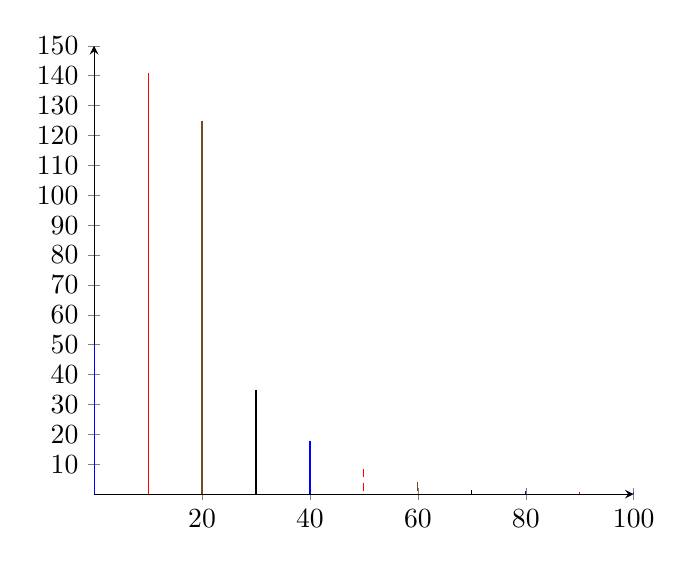
\begin{tikzpicture}
    \begin{axis}[
        xmin=0, xmax=100,
        ymin=0, ymax=150,
        axis lines=middle,
        ytick distance=10
      ]
      \path[name path=xaxis] (\pgfkeysvalueof{/pgfplots/xmin}, 0) -- (\pgfkeysvalueof{/pgfplots/xmax},0);
      \addplot +[mark=none] coordinates {(0, 50) (0, 0)};
      \addplot +[mark=none] coordinates {(10, 141) (10, 0)};
      \addplot +[mark=none] coordinates {(20, 125) (20, 0)};
      \addplot +[mark=none] coordinates {(30, 35) (30, 0)};
      \addplot +[mark=none] coordinates {(40, 17.7) (40, 0)};
      \addplot +[mark=none] coordinates {(50, 8.4) (50, 0)};
      \addplot +[mark=none] coordinates {(60, 3.95) (60, 0)};
      \addplot +[mark=none] coordinates {(70, 1.4) (70, 0)};
      \addplot +[mark=none] coordinates {(80, 1) (80, 0)};
      \addplot +[mark=none] coordinates {(90, 0.875) (90, 0)};
      \addplot +[mark=none] coordinates {(100, 0.7) (100, 0)};
    \end{axis}
  \end{tikzpicture}
\end{figure}
\end{document}